\documentclass[12pt]{article}

\usepackage{sbc-template}
\usepackage[utf8]{inputenc}
\usepackage[T1]{fontenc}
\usepackage[english,brazilian]{babel}
\usepackage{graphicx,url}
\usepackage{booktabs}
\usepackage{array}
\usepackage{amsmath}

\sloppy

% Números citados no texto, gerados por scripts/svm_report.py a partir de results/svm_dados.json.
% Gerado por scripts/svm_report.py a partir de report/results/svm_dados.json; não editar.
\newcommand{\svLinhasBrutas}{32.561}
\newcommand{\svPositivosBrutos}{24,1}
\newcommand{\svDuplicadas}{24}
\newcommand{\svAusentes}{2.398}
\newcommand{\svPositivosAusentes}{13,9}
\newcommand{\svLinhas}{30.139}
\newcommand{\svLinhasEn}{30,139}
\newcommand{\svPositivos}{24,9}
\newcommand{\svNPositivos}{7.506}
\newcommand{\svPiso}{75,1}
\newcommand{\svPisoEn}{75.1}
\newcommand{\svRazaoClasses}{3,0}
\newcommand{\svColunas}{80}
\newcommand{\svCorrFnlwgt}{$-$0,009}
\newcommand{\svPerfisConflito}{673}
\newcommand{\svLinhasConflito}{2.404}
\newcommand{\svPctConflito}{8}
\newcommand{\svErrosIrred}{867}
\newcommand{\svIrredPct}{2,9}
\newcommand{\svTeto}{97,1}
\newcommand{\svTetoEn}{97.1}
\newcommand{\svRepetemPerfil}{5.057}
\newcommand{\svCasados}{45,5}
\newcommand{\svNuncaCasou}{4,8}
\newcommand{\svEstudoNove}{16,4}
\newcommand{\svEstudoTreze}{42,2}
\newcommand{\svEstudoQuinze}{74,9}
\newcommand{\svCorrEstudo}{0,34}
\newcommand{\svCorrIdade}{0,24}
\newcommand{\svCorrHoras}{0,23}
\newcommand{\svCorrGanho}{0,22}
\newcommand{\svCorrPerda}{0,15}
\newcommand{\svGanhoMax}{99.999}
\newcommand{\svTreino}{24.111}
\newcommand{\svTeste}{6.028}
\newcommand{\svPositivosTeste}{1.501}
\newcommand{\svMargem}{30,4}
\newcommand{\svVetNeg}{4.232}
\newcommand{\svVetPos}{3.999}
\newcommand{\svKLinSVC}{84,6}
\newcommand{\svKSVCLin}{84,5}
\newcommand{\svKPoliDois}{85,0}
\newcommand{\svKPoliTres}{85,1}
\newcommand{\svKRBF}{84,9}
\newcommand{\svKAucLinSVC}{89,8}
\newcommand{\svKAucRBF}{89,1}
\newcommand{\svRazaoLinear}{59}
\newcommand{\svPadCom}{85,0}
\newcommand{\svPadSem}{80,6}
\newcommand{\svPadFCom}{67,6}
\newcommand{\svPadFSem}{50,8}
\newcommand{\svPadVetSem}{16.995}
\newcommand{\svPadVetSemPct}{70}
\newcommand{\svPadTempoSem}{29}
\newcommand{\svPadTempoCom}{6,6}
\newcommand{\svLinPadCom}{84,6}
\newcommand{\svLinPadSem}{84,6}
\newcommand{\svMapaMelhor}{85,45}
\newcommand{\svMapaMelhorC}{1}
\newcommand{\svMapaMelhorG}{0,3}
\newcommand{\svMapaPerto}{13}
\newcommand{\svMapaComb}{35}
\newcommand{\svMapaCanto}{75,1}
\newcommand{\svGammaUmTreino}{90,5}
\newcommand{\svGammaUmVal}{83,5}
\newcommand{\svMapaTempoMax}{41,6}
\newcommand{\svInclSVC}{1,93}
\newcommand{\svInclSVCLin}{1,95}
\newcommand{\svInclLinSVC}{1,05}
\newcommand{\svTempoSVC}{5,8}
\newcommand{\svTempoLinSVC}{0,07}
\newcommand{\svGTresAuc}{88,0}
\newcommand{\svGUmAuc}{89,7}
\newcommand{\svGTresAcc}{85,2}
\newcommand{\svGUmAcc}{85,5}
\newcommand{\svGTresSeeds}{5}
\newcommand{\svGUmSeeds}{4}
\newcommand{\svGTresVet}{9.232}
\newcommand{\svGUmVet}{8.340}
\newcommand{\svLinC}{0,1}
\newcommand{\svLinCSeeds}{7}
\newcommand{\svRBFCUmSeeds}{9}
\newcommand{\svPoliSeeds}{9}
\newcommand{\svArvComb}{8}
\newcommand{\svRedeComb}{10}
\newcommand{\svRedeEpMin}{33}
\newcommand{\svRedeEpMax}{86}
\newcommand{\svBuscaTotalRBF}{82}
\newcommand{\svBuscaTotalSVM}{104}
\newcommand{\svBuscaTotalRede}{17}
\newcommand{\svRecallRBF}{61}
\newcommand{\svRecallPesos}{85}
\newcommand{\svRBFPrevS}{2,0}
\newcommand{\svRazaoPrevRBFLin}{448}
\newcommand{\svRazaoPrevRBFRede}{361}
\newcommand{\svMajAcc}{75,1}
\newcommand{\svMajAccEn}{75.1}
\newcommand{\svMajSd}{0,0}
\newcommand{\svMajFum}{42,9}
\newcommand{\svMajFpos}{0,0}
\newcommand{\svMajAuc}{50,0}
\newcommand{\svMajAucEn}{50.0}
\newcommand{\svMajFP}{0}
\newcommand{\svMajFN}{1.501}
\newcommand{\svMajTreino}{0,01}
\newcommand{\svMajPrev}{4,3}
\newcommand{\svRegraAcc}{75,1}
\newcommand{\svRegraAccEn}{75.1}
\newcommand{\svRegraSd}{0,0}
\newcommand{\svRegraFum}{42,9}
\newcommand{\svRegraFpos}{0,0}
\newcommand{\svRegraAuc}{75,6}
\newcommand{\svRegraAucEn}{75.6}
\newcommand{\svRegraFP}{0}
\newcommand{\svRegraFN}{1.501}
\newcommand{\svRegraTreino}{0,02}
\newcommand{\svRegraPrev}{4,8}
\newcommand{\svLogAcc}{84,8}
\newcommand{\svLogAccEn}{84.8}
\newcommand{\svLogSd}{0,3}
\newcommand{\svLogFum}{78,3}
\newcommand{\svLogFpos}{66,5}
\newcommand{\svLogAuc}{90,2}
\newcommand{\svLogAucEn}{90.2}
\newcommand{\svLogFP}{325}
\newcommand{\svLogFN}{592}
\newcommand{\svLogTreino}{0,06}
\newcommand{\svLogPrev}{4,5}
\newcommand{\svArvAcc}{85,2}
\newcommand{\svArvAccEn}{85.2}
\newcommand{\svArvSd}{0,4}
\newcommand{\svArvFum}{78,4}
\newcommand{\svArvFpos}{66,4}
\newcommand{\svArvAuc}{90,0}
\newcommand{\svArvAucEn}{90.0}
\newcommand{\svArvFP}{277}
\newcommand{\svArvFN}{617}
\newcommand{\svArvTreino}{0,06}
\newcommand{\svArvPrev}{5,1}
\newcommand{\svArvBusca}{7,3}
\newcommand{\svRFAcc}{84,3}
\newcommand{\svRFAccEn}{84.3}
\newcommand{\svRFSd}{0,4}
\newcommand{\svRFFum}{78,1}
\newcommand{\svRFFpos}{66,5}
\newcommand{\svRFAuc}{89,1}
\newcommand{\svRFAucEn}{89.1}
\newcommand{\svRFFP}{391}
\newcommand{\svRFFN}{559}
\newcommand{\svRFTreino}{2,8}
\newcommand{\svRFPrev}{180}
\newcommand{\svLinAcc}{84,8}
\newcommand{\svLinAccEn}{84.8}
\newcommand{\svLinSd}{0,3}
\newcommand{\svLinFum}{78,2}
\newcommand{\svLinFpos}{66,2}
\newcommand{\svLinAuc}{90,2}
\newcommand{\svLinAucEn}{90.2}
\newcommand{\svLinFP}{311}
\newcommand{\svLinFN}{604}
\newcommand{\svLinTreino}{0,05}
\newcommand{\svLinPrev}{4,5}
\newcommand{\svLinBusca}{1,2}
\newcommand{\svRBFAcc}{85,4}
\newcommand{\svRBFAccEn}{85.4}
\newcommand{\svRBFSd}{0,4}
\newcommand{\svRBFFum}{79,0}
\newcommand{\svRBFFpos}{67,5}
\newcommand{\svRBFAuc}{88,9}
\newcommand{\svRBFAucEn}{88.9}
\newcommand{\svRBFFP}{294}
\newcommand{\svRBFFN}{587}
\newcommand{\svRBFTreino}{5,7}
\newcommand{\svRBFPrev}{2016}
\newcommand{\svRBFBusca}{8,0}
\newcommand{\svRBFVet}{8.764}
\newcommand{\svPoliAcc}{85,2}
\newcommand{\svPoliAccEn}{85.2}
\newcommand{\svPoliSd}{0,4}
\newcommand{\svPoliFum}{78,7}
\newcommand{\svPoliFpos}{66,9}
\newcommand{\svPoliAuc}{90,2}
\newcommand{\svPoliAucEn}{90.2}
\newcommand{\svPoliFP}{298}
\newcommand{\svPoliFN}{596}
\newcommand{\svPoliTreino}{3,6}
\newcommand{\svPoliPrev}{488}
\newcommand{\svPoliBusca}{2,2}
\newcommand{\svPoliVet}{8.128}
\newcommand{\svPesosAcc}{80,9}
\newcommand{\svPesosAccEn}{80.9}
\newcommand{\svPesosSd}{0,3}
\newcommand{\svPesosFum}{77,6}
\newcommand{\svPesosFpos}{69,0}
\newcommand{\svPesosAuc}{89,8}
\newcommand{\svPesosAucEn}{89.8}
\newcommand{\svPesosFP}{929}
\newcommand{\svPesosFN}{221}
\newcommand{\svPesosTreino}{6,3}
\newcommand{\svPesosPrev}{2283}
\newcommand{\svPesosVet}{9.995}
\newcommand{\svRedeAcc}{85,2}
\newcommand{\svRedeAccEn}{85.2}
\newcommand{\svRedeSd}{0,6}
\newcommand{\svRedeFum}{79,4}
\newcommand{\svRedeFpos}{68,4}
\newcommand{\svRedeAuc}{90,8}
\newcommand{\svRedeAucEn}{90.8}
\newcommand{\svRedeFP}{362}
\newcommand{\svRedeFN}{533}
\newcommand{\svRedeTreino}{1,0}
\newcommand{\svRedePrev}{5,6}
\newcommand{\svRedeBusca}{1,7}
\newcommand{\svDifRBFLinAcc}{+0,57}
\newcommand{\svSeedsRBFLinAcc}{10}
\newcommand{\svPRBFLinAcc}{0,002}
\newcommand{\svDifRBFLinFum}{+0,82}
\newcommand{\svSeedsRBFLinFum}{10}
\newcommand{\svPRBFLinFum}{0,002}
\newcommand{\svDifRBFLinAuc}{$-$1,31}
\newcommand{\svSeedsRBFLinAuc}{0}
\newcommand{\svPRBFLinAuc}{0,002}
\newcommand{\svDifRBFRFAcc}{+1,14}
\newcommand{\svSeedsRBFRFAcc}{10}
\newcommand{\svPRBFRFAcc}{0,002}
\newcommand{\svDifRBFRFFum}{+0,93}
\newcommand{\svSeedsRBFRFFum}{10}
\newcommand{\svPRBFRFFum}{0,002}
\newcommand{\svDifRBFRFAuc}{$-$0,25}
\newcommand{\svSeedsRBFRFAuc}{5}
\newcommand{\svPRBFRFAuc}{0,322}
\newcommand{\svDifRBFArvAcc}{+0,22}
\newcommand{\svSeedsRBFArvAcc}{6}
\newcommand{\svPRBFArvAcc}{0,160}
\newcommand{\svDifRBFArvFum}{+0,61}
\newcommand{\svSeedsRBFArvFum}{8}
\newcommand{\svPRBFArvFum}{0,037}
\newcommand{\svDifRBFArvAuc}{$-$1,09}
\newcommand{\svSeedsRBFArvAuc}{0}
\newcommand{\svPRBFArvAuc}{0,002}
\newcommand{\svDifPoliRBFAcc}{$-$0,23}
\newcommand{\svSeedsPoliRBFAcc}{2}
\newcommand{\svPPoliRBFAcc}{0,014}
\newcommand{\svDifPoliRBFFum}{$-$0,36}
\newcommand{\svSeedsPoliRBFFum}{1}
\newcommand{\svPPoliRBFFum}{0,006}
\newcommand{\svDifPoliRBFAuc}{+1,34}
\newcommand{\svSeedsPoliRBFAuc}{10}
\newcommand{\svPPoliRBFAuc}{0,002}
\newcommand{\svDifLinLogAcc}{+0,02}
\newcommand{\svSeedsLinLogAcc}{7}
\newcommand{\svPLinLogAcc}{0,369}
\newcommand{\svDifLinLogFum}{$-$0,13}
\newcommand{\svSeedsLinLogFum}{1}
\newcommand{\svPLinLogFum}{0,006}
\newcommand{\svDifLinLogAuc}{$-$0,02}
\newcommand{\svSeedsLinLogAuc}{3}
\newcommand{\svPLinLogAuc}{0,160}
\newcommand{\svDifRedeRBFAcc}{$-$0,22}
\newcommand{\svSeedsRedeRBFAcc}{2}
\newcommand{\svPRedeRBFAcc}{0,129}
\newcommand{\svDifRedeRBFFum}{+0,32}
\newcommand{\svSeedsRedeRBFFum}{7}
\newcommand{\svPRedeRBFFum}{0,105}
\newcommand{\svDifRedeRBFAuc}{+1,96}
\newcommand{\svSeedsRedeRBFAuc}{10}
\newcommand{\svPRedeRBFAuc}{0,002}
\newcommand{\svDifRedeLinAcc}{+0,35}
\newcommand{\svSeedsRedeLinAcc}{9}
\newcommand{\svPRedeLinAcc}{0,025}
\newcommand{\svDifRedeLinFum}{+1,14}
\newcommand{\svSeedsRedeLinFum}{10}
\newcommand{\svPRedeLinFum}{0,002}
\newcommand{\svDifRedeLinAuc}{+0,66}
\newcommand{\svSeedsRedeLinAuc}{10}
\newcommand{\svPRedeLinAuc}{0,002}
\newcommand{\svDifRedeArvAcc}{+-0,00}
\newcommand{\svSeedsRedeArvAcc}{5}
\newcommand{\svPRedeArvAcc}{0,941}
\newcommand{\svDifRedeArvFum}{+0,93}
\newcommand{\svSeedsRedeArvFum}{10}
\newcommand{\svPRedeArvFum}{0,002}
\newcommand{\svDifRedeArvAuc}{+0,88}
\newcommand{\svSeedsRedeArvAuc}{10}
\newcommand{\svPRedeArvAuc}{0,002}
\newcommand{\svDifRedePoliAcc}{+0,01}
\newcommand{\svSeedsRedePoliAcc}{5}
\newcommand{\svPRedePoliAcc}{1,000}
\newcommand{\svDifRedePoliFum}{+0,68}
\newcommand{\svSeedsRedePoliFum}{9}
\newcommand{\svPRedePoliFum}{0,010}
\newcommand{\svDifRedePoliAuc}{+0,62}
\newcommand{\svSeedsRedePoliAuc}{10}
\newcommand{\svPRedePoliAuc}{0,002}
\newcommand{\svDifRedeLogAcc}{+0,37}
\newcommand{\svSeedsRedeLogAcc}{9}
\newcommand{\svPRedeLogAcc}{0,027}
\newcommand{\svDifRedeLogFum}{+1,02}
\newcommand{\svSeedsRedeLogFum}{10}
\newcommand{\svPRedeLogFum}{0,002}
\newcommand{\svDifRedeLogAuc}{+0,64}
\newcommand{\svSeedsRedeLogAuc}{10}
\newcommand{\svPRedeLogAuc}{0,002}
\newcommand{\svDifRFArvAcc}{$-$0,92}
\newcommand{\svSeedsRFArvAcc}{0}
\newcommand{\svPRFArvAcc}{0,002}
\newcommand{\svDifRFArvFum}{$-$0,32}
\newcommand{\svSeedsRFArvFum}{3}
\newcommand{\svPRFArvFum}{0,232}
\newcommand{\svDifRFArvAuc}{$-$0,84}
\newcommand{\svSeedsRFArvAuc}{0}
\newcommand{\svPRFArvAuc}{0,002}
\newcommand{\svDifArvLogAcc}{+0,37}
\newcommand{\svSeedsArvLogAcc}{8}
\newcommand{\svPArvLogAcc}{0,019}
\newcommand{\svDifArvLogFum}{+0,09}
\newcommand{\svSeedsArvLogFum}{7}
\newcommand{\svPArvLogFum}{0,375}
\newcommand{\svDifArvLogAuc}{$-$0,24}
\newcommand{\svSeedsArvLogAuc}{2}
\newcommand{\svPArvLogAuc}{0,049}


\title{Máquinas de vetores de suporte na previsão de renda: kernels, custo e comparação com rede neural e modelos de referência}

\author{Bernan R. do Nascimento\inst{1}, Paulo E. R. Araujo\inst{1}, Thiago R. P. de Carvalho\inst{1}}

\address{Universidade Federal do Piauí (UFPI)\\
  Programa de Pós-Graduação em Ciência da Computação -- Teresina -- PI -- Brasil\\
  PPGCC010 -- Aprendizagem de Máquina (2026.2) -- Prof. Vinicius Ponte Machado
  \email{bernanr7@gmail.com, pauloaraujo@ufpi.edu.br}
  \email{thiago.rafael.pc@gmail.com}
}

\begin{document}

\maketitle

\begin{abstract}
  We predict whether a person's annual income exceeds 50 thousand dollars from 10 attributes of the
  1994 US census, on \svLinhasEn{} records of the Adult dataset, and use it to study the support vector
  machine (SVM) and compare it with simpler models and a neural network, including execution time.
  Identical profiles with different incomes cap any model at \svTetoEn\% accuracy. An RBF-kernel SVM
  reaches the best accuracy (\svRBFAccEn\%), less than one point above a linear boundary
  (\svLinAccEn\%), but a lower AUC than the linear SVM (\svRBFAucEn\% versus \svLinAucEn\%), because an
  accuracy-driven search picks a large gamma. The neural network matches it (\svRedeAccEn\%) with the
  best AUC (\svRedeAucEn\%) at a fraction of the cost.
\end{abstract}

\begin{resumo}
  Prevemos se a renda anual de uma pessoa passa de 50 mil dólares a partir de 10 atributos do censo dos
  EUA de 1994, em \svLinhas{} registros da base Adult, e a usamos para estudar a máquina de vetores de
  suporte (SVM) e compará-la com modelos mais simples e com uma rede neural, incluindo o tempo de
  execução. Perfis idênticos com rendas diferentes limitam qualquer modelo a \svTeto\% de acurácia. Sem
  padronização, a SVM com kernel RBF cai de \svPadCom\% para \svPadSem\%. Com ela, tem a melhor acurácia
  (\svRBFAcc\%), menos de um ponto acima de uma fronteira reta (\svLinAcc\%), mas AUC menor que a da SVM
  linear (\svRBFAuc\% contra \svLinAuc\%), porque a busca guiada pela acurácia escolhe um gamma alto. A
  rede neural chega ao mesmo nível (\svRedeAcc\%), com a melhor AUC (\svRedeAuc\%), a uma fração do custo.
\end{resumo}

\section{Introdução}

Este trabalho trata da previsão de renda: dada uma pessoa, descrita por 10 atributos do censo dos EUA de 1994, prever se a sua renda anual passa de 50 mil dólares. A base Adult~\cite{uci:adult,kohavi:96} tem cerca de 30 mil pessoas depois da curadoria. Nenhum atributo separa as classes sozinho, há atributos categóricos e valores ausentes, e o tamanho da base já torna visível o custo de treinar uma máquina de vetores de suporte (SVM)~\cite{boser:92,cortes:95} com kernel.

O modelo principal é a SVM, em quatro versões (linear, com kernel RBF, com kernel polinomial e RBF com pesos por classe), comparada com cinco modelos de referência (a classe majoritária, uma regra de um corte, a regressão logística, a árvore de decisão e a Random Forest) e com uma rede neural. Além da acurácia, registramos a AUC, os erros em cada classe e o tempo de treino, de busca de hiperparâmetros e de previsão de cada modelo. As contribuições são:
\begin{itemize}
  \item uma curadoria que mede o erro inevitável da base: perfis idênticos com rendas diferentes limitam qualquer modelo a \svTeto\% de acurácia (Seção~\ref{sec:sv_dados});
  \item um estudo da SVM numa divisão: kernels, o mapa de $C$ e $\gamma$, o efeito da padronização e o crescimento do tempo de treino com o tamanho da base (Seção~\ref{sec:sv_estudo});
  \item uma comparação em 10 seeds, com acurácia, F1, AUC, erros por classe e tempo num único núcleo, que mostra que a busca guiada pela acurácia piora a AUC da SVM com kernel RBF (Seção~\ref{sec:sv_seeds}).
\end{itemize}

\section{Fundamentação}

\textbf{Máquinas de vetores de suporte.} A SVM~\cite{boser:92,cortes:95} separa duas classes por um hiperplano $f(x) = w \cdot x + b$, respondendo a classe positiva quando $f(x) > 0$. Entre os hiperplanos que separam o treino, ela escolhe o de maior margem, a faixa vazia entre a fronteira e os pontos mais próximos de cada classe, de largura $2/\lVert w \rVert$. Como dados reais raramente se separam por completo, a formulação de margem suave aceita pontos dentro da margem ou do lado errado, cobrando por eles a perda \emph{hinge}:
\begin{equation*}
  \min_{w,\,b} \; \tfrac{1}{2}\lVert w \rVert^2 + C \sum_i \max\bigl(0,\; 1 - y_i\, f(x_i)\bigr), \qquad y_i \in \{-1, +1\}.
\end{equation*}
O hiperparâmetro $C$ pesa os erros contra a largura da margem: $C$ pequeno tolera erros e deixa a fronteira simples; $C$ grande tenta acertar todo o treino. A solução depende só dos pontos com perda positiva ou sobre a margem, os \emph{vetores de suporte}. A SVM não estima probabilidades: sua saída é a distância com sinal até a fronteira, que serve para ordenar exemplos e calcular a AUC. Probabilidades exigem uma calibração à parte~\cite{platt:99}.

\textbf{Kernels.} No problema dual, os dados aparecem só em produtos $x_i \cdot x_j$. Trocar esse produto por um kernel $K(x_i, x_j)$ equivale a traçar o hiperplano num espaço transformado, sem calculá-lo, e a fronteira no espaço original fica curva: $f(x) = \sum_i \alpha_i y_i K(x_i, x) + b$, com a soma sobre os vetores de suporte. Usamos o kernel polinomial, $(\gamma\, x \cdot x' + c_0)^d$, e o RBF, $\exp(-\gamma \lVert x - x' \rVert^2)$. No RBF, $\gamma$ controla o alcance de cada vetor de suporte: pequeno, a fronteira é suave; grande, ela contorna os pontos do treino. Como o RBF mede distâncias, atributos em escalas diferentes precisam ser padronizados~\cite{hsu:03}. O treino pelo LIBSVM~\cite{chang:11} trabalha com pares de exemplos, e seu custo cresce entre o quadrado e o cubo do tamanho do treino; a previsão compara cada exemplo novo com todos os vetores de suporte. Para o kernel linear, o LIBLINEAR~\cite{fan:08} otimiza diretamente os pesos $w$, com custo proporcional ao tamanho do treino.

\textbf{Redes neurais.} Um neurônio artificial calcula uma soma ponderada das entradas, mais um viés, e aplica a ela uma função de ativação. Com a sigmoide, que leva qualquer número a um valor entre 0 e 1, um único neurônio é a regressão logística. O perceptron de múltiplas camadas (MLP) empilha camadas de neurônios entre a entrada e a saída, as camadas ocultas; com a ativação ReLU, $\max(0, z)$~\cite{nair:10}, elas permitem fronteiras de decisão não lineares. Os pesos começam sorteados e são ajustados pela retropropagação do erro~\cite{rumelhart:86}: a cada lote de exemplos, calcula-se quanto cada peso contribuiu para a perda (aqui, a entropia cruzada) e move-se o peso no sentido de reduzi-la, com um passo dado pela taxa de aprendizado. O otimizador Adam~\cite{kingma:15} adapta esse passo para cada peso. Uma época é uma passada completa pelo treino. Como o passo é o mesmo para entradas de escalas muito diferentes, os atributos costumam ser padronizados antes~\cite{lecun:98}. Treinar por épocas demais leva a rede a se ajustar a detalhes do treino; a parada antecipada~\cite{prechelt:98} separa uma parte do treino como validação e interrompe o treino quando o desempenho nela para de melhorar. Ao contrário da SVM, a rede é treinada para estimar probabilidades. Em dados tabulares, modelos de árvore ainda costumam superar redes neurais~\cite{grinsztajn:22}.

\textbf{Modelos de referência.} O CART~\cite{breiman:84} divide o espaço de atributos de forma recursiva, em cada nó escolhendo o limiar de um atributo que mais reduz a impureza (Gini ou entropia); a vantagem é a legibilidade das regras. Uma árvore de profundidade 1 é uma \emph{regra de um corte}: um único atributo comparado com um único limiar. A Random Forest~\cite{breiman:01} treina muitas árvores, cada uma numa amostra com reposição do treino (\emph{bootstrap}) e com sorteio dos atributos de cada nó, e a previsão é a média dos votos. A regressão logística, como visto acima, equivale a uma rede de um único neurônio.

\section{Dados e curadoria}\label{sec:sv_dados}

A base Adult~\cite{uci:adult} foi extraída do censo dos EUA de 1994 por Barry Becker e doada à UCI por Becker e Kohavi~\cite{kohavi:96}. A versão do Kaggle~\cite{kaggle:adult} tem \svLinhasBrutas{} registros, um por pessoa, com 14 atributos e o rótulo \texttt{income}, que diz se a renda anual passa de 50 mil dólares (\svPositivosBrutos\% passam). O arquivo é conferido pelo seu \emph{hash} SHA-256, para garantir que todos os experimentos partem do mesmo arquivo. A Tabela~\ref{tab:sv_atributos} lista os 10 atributos usados, com os nomes deste trabalho.

\begin{table}[ht]
\centering
\caption{Atributos usados: nome no arquivo original, nome neste trabalho e valores, após a curadoria.}
\label{tab:sv_atributos}
\footnotesize
\begin{tabular}{lll}
\toprule
Coluna original & Nome neste trabalho & Valores \\
\midrule
\texttt{age} & idade & 17 a 90 anos \\
\texttt{education.num} & anos de estudo & 1 a 16 \\
\texttt{capital.gain} & ganho de capital & 0 a \svGanhoMax{} dólares \\
\texttt{capital.loss} & perda de capital & 0 a 4.356 dólares \\
\texttt{hours.per.week} & horas por semana & 1 a 99 \\
\texttt{workclass} & classe de trabalho & 7 categorias \\
\texttt{marital.status} & estado civil & 7 categorias \\
\texttt{occupation} & ocupação & 14 categorias \\
\texttt{relationship} & relacionamento & 6 categorias \\
\texttt{native.country} & país de origem & 41 países \\
\texttt{income} & renda acima de 50 mil (rótulo) & 1 = \texttt{>50K}, 0 = \texttt{<=50K} \\
\bottomrule
\end{tabular}
\end{table}

\textbf{Linhas.} \svDuplicadas{} linhas eram cópias exatas de outras, inclusive no peso amostral, e foram removidas. Outras \svAusentes{} tinham valor ausente, marcado com ``?'', quase sempre na classe de trabalho e na ocupação ao mesmo tempo, ou no país. Nessas linhas, \svPositivosAusentes\% ganham mais de 50 mil, contra \svPositivos\% no resto; como são 7\% da base e preencher a ocupação inventaria um dado num dos atributos mais informativos, foram removidas. Restam \svLinhas{} pessoas, \svPositivos\% com renda acima de 50 mil.

\textbf{Atributos.} O \texttt{fnlwgt} é um peso amostral, quantas pessoas da população cada registro representa, e não uma característica da pessoa; sua correlação com o rótulo é de \svCorrFnlwgt, e ele foi removido. O \texttt{education} é a escolaridade em texto e corresponde, nível a nível, ao \texttt{education.num}; ficou só o número. Raça e sexo foram mantidos no arquivo, mas ficaram fora dos atributos de todos os modelos. Foi uma decisão do grupo: o objetivo do trabalho é estudar a SVM, e não queríamos um modelo que usasse raça ou sexo para prever a renda de alguém. Isso não garante, porém, que o modelo ignore essas características (Seção~\ref{sec:limitacoes}).

\textbf{Perfis repetidos e erro inevitável.} Sem o peso amostral, pessoas diferentes passam a ter os mesmos 10 atributos: \svRepetemPerfil{} linhas repetem o perfil de outra. \svPerfisConflito{} desses perfis aparecem com as duas rendas, em \svLinhasConflito{} linhas (\svPctConflito\% da base). Qualquer modelo dá a mesma resposta a pessoas com os mesmos dados; o melhor possível é responder, em cada perfil, a renda mais comum, o que deixa no mínimo \svErrosIrred{} erros (\svIrredPct\% da base). Nenhum modelo pode, portanto, passar de \svTeto\% de acurácia.

\section{Análise exploratória}\label{sec:sv_eda}

\svPositivos\% das pessoas ganham mais de 50 mil, cerca de \svRazaoClasses{} pessoas abaixo para cada uma acima: responder sempre ``até 50 mil'' já acerta \svPiso\%, e esse é o piso. Entre os numéricos, os anos de estudo têm a maior correlação com o rótulo (\svCorrEstudo), seguidos da idade (\svCorrIdade), das horas por semana (\svCorrHoras), do ganho de capital (\svCorrGanho) e da perda de capital (\svCorrPerda). Entre os categóricos, o estado civil é o que mais separa: entre os casados, \svCasados\% ganham mais de 50 mil; entre quem nunca casou, \svNuncaCasou\% (Figura~\ref{fig:sv_eda}a). A renda alta cresce com os anos de estudo: \svEstudoNove\% com 9 anos, \svEstudoTreze\% com 13 e \svEstudoQuinze\% com 15 (Figura~\ref{fig:sv_eda}b).

\begin{figure}[ht]
\centering
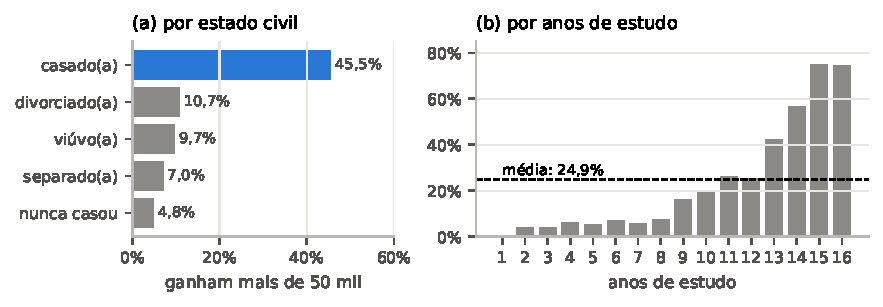
\includegraphics[width=\textwidth]{figures/svm_eda.pdf}
\caption{Proporção de pessoas que ganham mais de 50 mil (a) por estado civil, nas cinco categorias mais comuns, e (b) por anos de estudo, na base inteira (\svLinhas{} pessoas). A linha tracejada é a proporção geral.}
\label{fig:sv_eda}
\end{figure}


Mesmo o atributo mais forte não basta: nem entre os casados a renda alta passa da metade. Separar as classes exige, portanto, combinar vários atributos, e a distância entre o piso (\svPiso\%) e o teto (\svTeto\%) é o espaço em que os modelos competem.

\section{Metodologia}\label{sec:sv_metodo}

\textbf{Pré-processamento.} Os cinco atributos categóricos viram colunas 0/1, uma por categoria (\emph{one-hot}), e os cinco numéricos são padronizados (subtrai-se a média e divide-se pelo desvio padrão). São \svColunas{} colunas no total. Codificação, padronização e modelo ficam num único \emph{pipeline} do scikit-learn~\cite{pedregosa:11}, de modo que a média e o desvio vêm só do treino de cada divisão, e de cada parte da validação cruzada.

\textbf{Protocolo.} Os dados são divididos em treino (80\%, \svTreino{} pessoas) e teste (20\%, \svTeste, das quais \svPositivosTeste{} acima de 50 mil), mantendo a proporção das classes, e o procedimento é repetido com 10 seeds (0 a 9), que mudam a divisão, as partes da validação cruzada e a semente dos modelos. Quando um modelo tem hiperparâmetros, uma busca em grade com validação cruzada estratificada de 5 partes, só no treino, escolhe a combinação de maior acurácia, e o modelo é treinado de novo no treino inteiro. No teste, reportam-se a acurácia, o F1 macro (média do F1 das duas classes), o F1 da classe acima de 50 mil, a AUC e os falsos positivos e negativos, com a classe acima de 50 mil como positiva. A AUC usa a probabilidade prevista ou, na SVM, a distância à fronteira: mede se o modelo ordena bem as pessoas, independentemente do corte.

\textbf{Modelos.} As referências são a classe majoritária; a regra de um corte, uma árvore de profundidade 1 que escolhe sozinha, no treino, o melhor atributo e o melhor limiar; a regressão logística; a árvore de decisão com busca em grade; e a Random Forest com 300 árvores. A SVM aparece em quatro versões: a SVM linear, pelo LIBLINEAR (\texttt{LinearSVC}); a SVM com kernel RBF e a com kernel polinomial ($c_0 = 1$), pelo LIBSVM (\texttt{SVC}); e a SVM RBF com pesos por classe (\texttt{class\_weight="balanced"}, que faz o erro na classe menor custar cerca de 3 vezes mais), com os $C$ e $\gamma$ escolhidos para a RBF em cada seed. A rede neural é um MLP do scikit-learn: camadas ocultas com ativação ReLU, um neurônio de saída com sigmoide, perda de entropia cruzada e otimizador Adam, com parada antecipada (10\% do treino ficam de fora como validação, e o treino para depois de 30 épocas sem melhora). A busca da rede cobre a arquitetura (8, 16, 32 ou 64 neurônios numa camada; 32 e 16 ou 64 e 32 em duas), a regularização L2 e a taxa de aprendizado. As grades da SVM saíram de um estudo numa única divisão (a seed 0), apresentado na Seção~\ref{sec:sv_estudo}; a Tabela~\ref{tab:sv_grades} reúne todas.

\begin{table}[ht]
\centering
\caption{Grades da busca (número de combinações após os dois-pontos) e o que a busca escolheu nas 10 seeds.}
\label{tab:sv_grades}
\footnotesize
\begin{tabular}{l>{\raggedright\arraybackslash}p{5.6cm}>{\raggedright\arraybackslash}p{4.2cm}}
\toprule
Modelo & Valores testados & Escolha nas 10 seeds \\
\midrule
Árvore de decisão & critério (Gini, entropia) $\times$ profundidade (3, 5, 8, 12, sem limite) $\times$ mínimo por folha (1, 5, 20): 30 & 8 combinações diferentes; profundidade de 8 para cima ou sem limite \\
SVM linear & C $\in$ \{0,001; 0,01; 0,1; 1; 10\}: 5 & C = 0,1 em 7 \\
SVM RBF & C $\in$ \{0,1; 1; 10; 100\} $\times$ $\gamma$ $\in$ \{0,01; 0,03; 0,1; 0,3\}: 16 & C = 1 em 9, com $\gamma$ = 0,3 (5) ou 0,1 (4); C = 10 e $\gamma$ = 0,03 em 1 \\
SVM polinomial & grau $\in$ \{2; 3\} $\times$ C $\in$ \{0,1; 1; 10\}, coef0 = 1: 6 & grau 2 e C = 1 em 9 \\
Rede neural & 6 arquiteturas $\times$ $\alpha$ (10$^{-4}$, 10$^{-2}$) $\times$ taxa (10$^{-3}$, 10$^{-2}$): 24 & 10 combinações diferentes \\
\bottomrule
\end{tabular}

\end{table}

\textbf{Tempo de execução.} Para comparar algoritmos, e não o número de núcleos que cada um usa, tudo roda num único núcleo (\texttt{n\_jobs=1} e as bibliotecas de álgebra linear limitadas a uma \emph{thread}), com uma rodada de aquecimento descartada. Nos modelos com busca, o tempo da busca é medido à parte do treino final. O resumo usa a mediana das 10 seeds. A máquina é um AMD Ryzen 5 9600X (6 núcleos) com 31 GB de memória, Windows 11 e scikit-learn 1.9.1.

\section{Resultados}\label{sec:sv_resultados}

\subsection{Estudo da SVM numa divisão}\label{sec:sv_estudo}

Na seed 0, a SVM RBF com $C = 1$ e o $\gamma$ padrão do scikit-learn usa \svVetNeg{} vetores de suporte da classe até 50 mil e \svVetPos{} da classe acima: a classe menor, um quarto do treino, é metade dos vetores, porque boa parte dela fica perto da fronteira. \svMargem\% das pessoas do teste caem dentro da margem, com distância à fronteira entre $-1$ e $+1$.

\textbf{Kernels.} Com $C = 1$ e sem ajuste, os cinco modelos da Tabela~\ref{tab:sv_seed0} ficam entre \svKSVCLin\% e \svKPoliTres\% de acurácia; as fronteiras curvas ganham cerca de meio ponto das retas. A LinearSVC e a SVC com kernel linear chegam à mesma fronteira (\svKLinSVC\% e \svKSVCLin\%), mas a LinearSVC treina cerca de \svRazaoLinear{} vezes mais rápido, e por isso é a SVM linear das comparações seguintes. Na AUC a ordem já se inverte: \svKAucLinSVC\% para a LinearSVC, \svKAucRBF\% para a RBF.

\begin{table}[ht]
\centering
\caption{Seed 0: os kernels com $C = 1$ e o efeito da padronização (\svTreino{} pessoas no treino, \svTeste{} no teste).}
\label{tab:sv_seed0}
\footnotesize
\begin{tabular}{lccc}
\toprule
Modelo (seed 0) & Acurácia (\%) & AUC (\%) & Treino (s) \\
\midrule
\multicolumn{4}{l}{\emph{Kernels, com C = 1}} \\
SVM linear (LinearSVC) & 84,6 & 89,8 & 0,08 \\
SVC, kernel linear & 84,5 & 89,7 & 4,62 \\
SVC polinomial, grau 2 & 85,0 & 89,9 & 3,97 \\
SVC polinomial, grau 3 & 85,1 & 88,8 & 5,06 \\
SVC RBF & 84,9 & 89,1 & 4,82 \\
\midrule
\multicolumn{4}{l}{\emph{Padronização (RBF com C = 1 e $\gamma$ = 0,3; LinearSVC com C = 1)}} \\
RBF, com padronização & 85,0 & 87,6 & 6,62 \\
RBF, sem padronização & 80,6 & 82,4 & 28,96 \\
LinearSVC, com padronização & 84,6 & 89,8 & 0,08 \\
LinearSVC, sem padronização & 84,6 & 89,6 & 0,07 \\
\bottomrule
\end{tabular}

\end{table}

\textbf{C e $\gamma$.} A Figura~\ref{fig:sv_mapa} mostra a acurácia de validação cruzada da SVM RBF em 5 valores de $C$ e 7 de $\gamma$ (175 treinos). A melhor combinação, $C = \svMapaMelhorC$ e $\gamma = \svMapaMelhorG$, chega a \svMapaMelhor\%, mas \svMapaPerto{} das \svMapaComb{} combinações ficam a até meio ponto dela: os bons resultados formam um platô na diagonal, em que um $\gamma$ menor pede um $C$ maior. Os dois compensam um ao outro: $\gamma$ pequeno deixa a fronteira suave, e $C$ grande a obriga a se ajustar mais. Nos cantos o modelo falha. Com $C$ e $\gamma$ pequenos, responde ``até 50 mil'' para quase todos (\svMapaCanto\%, o piso). Com $\gamma = 1$, sobreajusta em qualquer $C$: a acurácia no treino chega a \svGammaUmTreino\%, e a de validação cai para \svGammaUmVal\% (Figura~\ref{fig:sv_gamma}). A grade das 10 seeds cobre o platô e deixa de fora esses cantos (Tabela~\ref{tab:sv_grades}).

\begin{figure}[ht]
\centering
\begin{minipage}[b]{.55\textwidth}
\centering
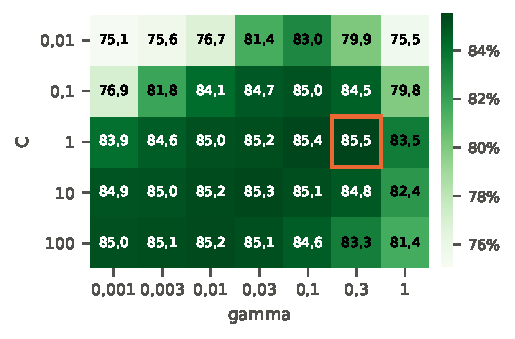
\includegraphics[width=\textwidth]{figures/svm_mapa.pdf}
\caption{Acurácia de validação cruzada (5 partes, seed 0) da SVM RBF por $C$ e $\gamma$. O quadro marca a melhor combinação.}
\label{fig:sv_mapa}
\end{minipage}\hfill
\begin{minipage}[b]{.42\textwidth}
\centering
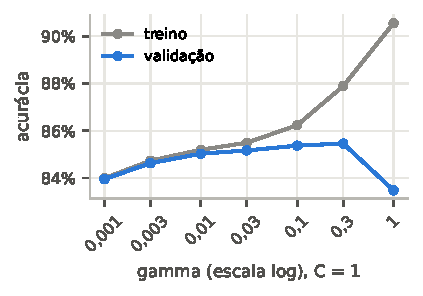
\includegraphics[width=\textwidth]{figures/svm_gamma.pdf}
\caption{Acurácia no treino e na validação por $\gamma$, com $C = 1$ (seed 0).}
\label{fig:sv_gamma}
\end{minipage}
\end{figure}

\textbf{Padronização.} Sem padronização, a SVM RBF cai de \svPadCom\% para \svPadSem\% de acurácia, e o F1 da classe acima de 50 mil, de \svPadFCom\% para \svPadFSem\%; o modelo passa a usar \svPadVetSem{} vetores de suporte (\svPadVetSemPct\% do treino) e leva \svPadTempoSem{} s para treinar, contra \svPadTempoCom{} s (Tabela~\ref{tab:sv_seed0}). O kernel RBF mede a distância entre pessoas somando as diferenças em todos os atributos, e o ganho de capital, que vai até \svGanhoMax, domina essa soma quando não é padronizado~\cite{hsu:03}. A LinearSVC não muda (\svLinPadCom\% e \svLinPadSem\%): o modelo linear dá um peso a cada atributo, e um atributo de escala grande só recebe um peso menor.

\textbf{Tempo por tamanho do treino.} A Figura~\ref{fig:sv_tempo} mede o tempo de treino de cada modelo com 1.000 a \svTreino{} pessoas. Em escala log, a inclinação da reta diz como o tempo cresce. A da SVC é \svInclSVC{} com kernel RBF e \svInclSVCLin{} com kernel linear: dobrar o treino quadruplica o tempo. A da LinearSVC é \svInclLinSVC, tempo proporcional ao treino. Com o treino inteiro, a SVC RBF leva \svTempoSVC{} s, e a LinearSVC, \svTempoLinSVC{} s. A Random Forest é mais lenta que a SVC nos tamanhos pequenos, mas as curvas se cruzam entre 8 e 16 mil pessoas. Pela mesma inclinação, a SVC levaria cerca de 100 s com 100 mil pessoas e horas com um milhão.

\begin{figure}[ht]
\centering
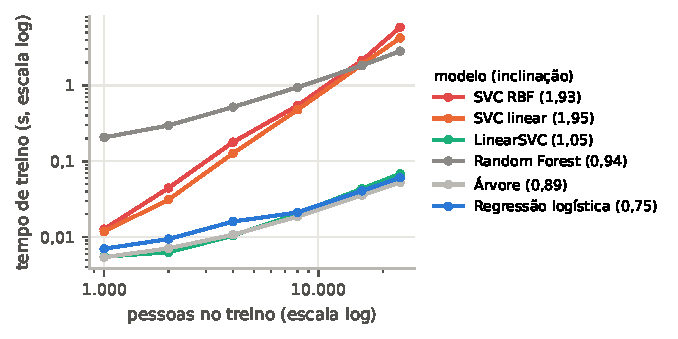
\includegraphics[width=.8\textwidth]{figures/svm_tempo.pdf}
\caption{Tempo de treino (um núcleo, seed 0) por número de pessoas no treino, em escala log nos dois eixos. Entre parênteses, a inclinação da reta ajustada de 4.000 pessoas para cima.}
\label{fig:sv_tempo}
\end{figure}

\subsection{Comparação em 10 seeds}\label{sec:sv_seeds}

A Tabela~\ref{tab:sv_modelos} e a Figura~\ref{fig:sv_acc_auc} reúnem os dez modelos. Nas referências, a regressão logística (\svLogAcc\%) e a árvore ajustada (\svArvAcc\%) ficam a menos de meio ponto uma da outra, e a Random Forest (\svRFAcc\%) fica abaixo da árvore em todas as seeds (\svDifRFArvAcc{} ponto): na configuração padrão, cada árvore cresce até folhas de uma pessoa e decora o ruído dos perfis em conflito. A regra de um corte pergunta, nas 10 seeds, se a pessoa é casada, mas responde ``até 50 mil'' dos dois lados e empata com o piso; sua AUC de \svRegraAuc\% mostra que a pergunta ordena bem as pessoas, e o que falha é o corte. Todos os modelos sem pesos erram cerca de duas vezes mais por falso negativo do que por falso positivo.

\begin{table}[ht]
\centering
\caption{Os dez modelos na base de renda (média $\pm$ desvio em 10 seeds; FP e FN: falsos positivos e negativos em \svTeste{} pessoas de teste, \svPositivosTeste{} delas acima de 50 mil). Tempos: mediana das 10 seeds, num único núcleo; treino do modelo final e previsão do teste inteiro.}
\label{tab:sv_modelos}
\footnotesize
\setlength{\tabcolsep}{3.5pt}
\begin{tabular}{lcccccccc}
\toprule
Modelo & Acurácia (\%) & \shortstack{F1 macro\\(\%)} & \shortstack{F1 $>$50K\\(\%)} & AUC (\%) & FP & FN & \shortstack{Treino\\(s)} & \shortstack{Previsão\\(ms)} \\
\midrule
Classe majoritária & 75,1 $\pm$ 0,0 & 42,9 & 0,0 & 50,0 & 0 & 1.501 & 0,01 & 4,3 \\
Regra de um corte & 75,1 $\pm$ 0,0 & 42,9 & 0,0 & 75,6 & 0 & 1.501 & 0,02 & 4,8 \\
Regressão logística & 84,8 $\pm$ 0,3 & 78,3 & 66,5 & 90,2 & 325 & 592 & 0,06 & 4,5 \\
Árvore de decisão & 85,2 $\pm$ 0,4 & 78,4 & 66,4 & 90,0 & 277 & 617 & 0,06 & 5,1 \\
Random Forest & 84,3 $\pm$ 0,4 & 78,1 & 66,5 & 89,1 & 391 & 559 & 2,8 & 180 \\
\midrule
SVM linear & 84,8 $\pm$ 0,3 & 78,2 & 66,2 & 90,2 & 311 & 604 & 0,05 & 4,5 \\
SVM RBF & 85,4 $\pm$ 0,4 & 79,0 & 67,5 & 88,9 & 294 & 587 & 5,7 & 2016 \\
SVM polinomial & 85,2 $\pm$ 0,4 & 78,7 & 66,9 & 90,2 & 298 & 596 & 3,6 & 488 \\
SVM RBF com pesos & 80,9 $\pm$ 0,3 & 77,6 & 69,0 & 89,8 & 929 & 221 & 6,3 & 2283 \\
Rede neural (MLP) & 85,2 $\pm$ 0,6 & 79,4 & 68,4 & 90,8 & 362 & 533 & 1,0 & 5,6 \\
\bottomrule
\end{tabular}

\end{table}

\begin{figure}[ht]
\centering
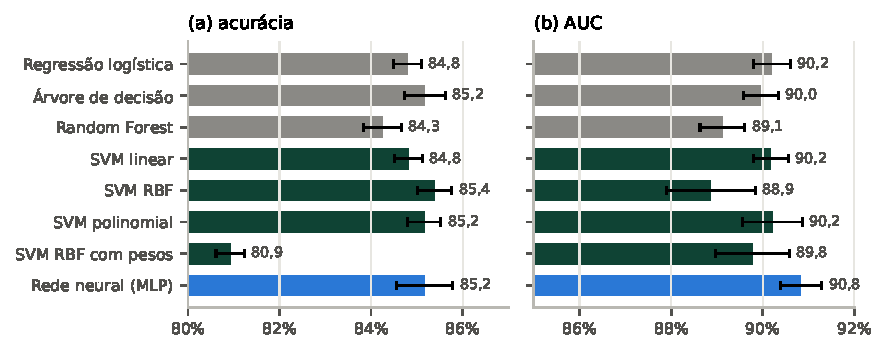
\includegraphics[width=\textwidth]{figures/svm_acc_auc.pdf}
\caption{(a) Acurácia e (b) AUC no teste, média e desvio de 10 seeds. Os eixos começam em 80\% e 85\%. Em verde-escuro, as SVMs.}
\label{fig:sv_acc_auc}
\end{figure}

\textbf{A SVM.} A SVM RBF tem a melhor acurácia, \svRBFAcc~$\pm$~\svRBFSd\%, e o melhor F1 macro entre as SVMs (\svRBFFum\%). Comparando seed a seed, supera a SVM linear em \svSeedsRBFLinAcc{} das 10 seeds (\svDifRBFLinAcc{} ponto) e a Random Forest em \svSeedsRBFRFAcc{} (\svDifRBFRFAcc), mas contra a árvore ajustada fica à frente em só \svSeedsRBFArvAcc{} (\svDifRBFArvAcc{} ponto, menos que o desvio entre seeds): é um empate (teste de Wilcoxon pareado, $p = \svPRBFArvAcc$; contra a SVM linear, $p = \svPRBFLinAcc$, o menor valor possível com 10 seeds). As 10 divisões compartilham os mesmos dados, então os valores de $p$ são otimistas e servem só para separar empate de diferença. A SVM polinomial, de grau 2 em quase todas as seeds, fica entre as duas (\svPoliAcc\%). A SVM linear e a regressão logística são, na prática, o mesmo modelo: \svDifLinLogAcc{} ponto de diferença. A fronteira curva rende, portanto, menos de um ponto sobre a reta, longe do teto de \svTeto\%. A busca foi estável: a SVM RBF escolheu $C = 1$ em \svRBFCUmSeeds{} seeds e a linear, $C = \svLinC$ em \svLinCSeeds{} (Tabela~\ref{tab:sv_grades}).

\textbf{Acurácia contra AUC.} Na AUC a ordem se inverte: a SVM RBF tem \svRBFAuc\%, abaixo da SVM linear e da polinomial (\svLinAuc\% e \svPoliAuc\%), e perde para a linear em todas as seeds (\svDifRBFLinAuc{} ponto). A causa é o critério da busca. A acurácia só olha de que lado da fronteira cada pessoa cai; a AUC olha a ordem das notas. Guiada pela acurácia, a busca prefere $\gamma$ alto, que ajusta bem a fronteira; mas com $\gamma$ alto cada vetor de suporte só influencia a sua vizinhança, e longe deles a nota de quase todos se aproxima do mesmo valor, o que desfaz a ordem entre as pessoas longe da fronteira. Nas \svGTresSeeds{} seeds em que a busca escolheu $\gamma = 0{,}3$, a AUC foi \svGTresAuc\%; nas \svGUmSeeds{} com $\gamma = 0{,}1$, \svGUmAuc\%. E a acurácia no teste nem foi maior com $\gamma = 0{,}3$ (\svGTresAcc\% contra \svGUmAcc\%): a preferência veio de décimos na validação que não se repetiram no teste. Para ordenar pessoas por chance de renda alta, a busca deveria usar a AUC como critério.

\textbf{Pesos por classe.} Com os mesmos $C$ e $\gamma$, os pesos por classe reduzem os falsos negativos de \svRBFFN{} para \svPesosFN: o modelo passa a encontrar \svRecallPesos\% das pessoas de renda alta, contra \svRecallRBF\%. Em troca, os falsos positivos sobem de \svRBFFP{} para \svPesosFP, e a acurácia cai para \svPesosAcc\%. O F1 da classe acima de 50 mil é o maior de todos (\svPesosFpos\%). Qual versão usar depende do custo de cada erro.

\textbf{A rede neural.} A rede chega a \svRedeAcc~$\pm$~\svRedeSd\%, com o melhor F1 macro (\svRedeFum\%) e a melhor AUC (\svRedeAuc\%) dos dez modelos. Na acurácia, a rede supera a SVM RBF em só \svSeedsRedeRBFAcc{} das 10 seeds (\svDifRedeRBFAcc{} ponto); no F1 macro, em \svSeedsRedeRBFFum{} (\svDifRedeRBFFum), um empate; na AUC, em todas (\svDifRedeRBFAuc{} pontos, $p = \svPRedeRBFAuc$; na acurácia, $p = \svPRedeRBFAcc$, e no F1 macro, $p = \svPRedeRBFFum$), e também supera todos os outros modelos na AUC em todas as seeds. A rede é treinada para estimar probabilidades, e suas notas ordenam bem as pessoas em toda a faixa; a SVM só aprende o lado da fronteira. Em troca, varia mais entre seeds: a busca escolheu \svRedeComb{} combinações diferentes em 10 seeds, e a parada antecipada interrompeu o treino entre \svRedeEpMin{} e \svRedeEpMax{} épocas.

\textbf{Tempo.} A SVM com kernel é cara duas vezes. O treino final da SVM RBF leva \svRBFTreino{} s, contra \svLinTreino{} s da SVM linear e \svRedeTreino{} s da rede, e a busca leva \svRBFBusca{} min por seed, contra \svRedeBusca{} min da rede; nas 10 seeds, \svBuscaTotalRBF{} minutos só na busca da SVM RBF. Prever o teste leva \svRBFPrevS{} s, cerca de \svRazaoPrevRBFLin{} vezes a SVM linear e \svRazaoPrevRBFRede{} vezes a rede, porque cada pessoa é comparada com os vetores de suporte (\svRBFVet{}, em média), enquanto a SVM linear e a rede só multiplicam a pessoa por pesos fixos.

\section{Limitações}\label{sec:limitacoes}

A curadoria removeu as \svAusentes{} linhas com valor ausente. Elas ganham mais de 50 mil com menos frequência (\svPositivosAusentes\% contra \svPositivos\%), de modo que a base ficou um pouco mais ``rica'' e os modelos não aprenderam o perfil de quem está fora do mercado de trabalho ou tem vínculo informal. Tratar o ausente como uma categoria própria manteria essas pessoas; não medimos quanto isso mudaria os resultados.

As grades da SVM foram escolhidas a partir de um estudo numa única divisão, a seed 0, que também faz parte das 10 seeds da comparação; o mapa de $C$ e $\gamma$ é largo e plano o bastante para que isso pese pouco, mas a escolha não foi independente da avaliação. A busca usou a acurácia como critério em todos os modelos, e a Seção~\ref{sec:sv_seeds} mostra que esse critério piora a AUC da SVM RBF; com a AUC como critério, a comparação poderia mudar. A Random Forest foi usada na configuração padrão, sem ajuste. As 10 seeds variam o sorteio da divisão, mas os dados são os mesmos, de modo que o desvio padrão não mede a incerteza para dados novos. Os tempos foram medidos numa única máquina, num núcleo só; os valores absolutos mudam com o computador, e as razões entre modelos são mais estáveis que os tempos em si.

Deixar raça e sexo fora dos atributos não impede que o modelo aprenda padrões ligados a eles: outros atributos carregam a mesma informação, como o relacionamento, em que ``marido'' e ``esposa'' indicam o sexo quase sem exceção. Não avaliamos aqui os efeitos disso. A base é de 1994, e o limite de 50 mil dólares, de outro tempo; as conclusões valem para esta base.

\section{Conclusão e trabalhos futuros}

Na base Adult, com \svLinhas{} pessoas e um teto de \svTeto\% imposto por perfis idênticos com rendas diferentes, a SVM com kernel RBF tem a melhor acurácia, \svRBFAcc~$\pm$~\svRBFSd\%: supera a SVM linear e a Random Forest nas 10 seeds, mas empata com a árvore ajustada, e a vantagem sobre uma fronteira reta é de menos de um ponto. O estudo numa divisão mostrou o que a SVM exige: padronização (sem ela, \svPadSem\%), um par de $C$ e $\gamma$ dentro de um platô largo, e um tempo de treino que cresce com o quadrado do tamanho do treino. A busca guiada pela acurácia escolhe um $\gamma$ alto, que dá à SVM RBF a pior AUC entre as SVMs (\svRBFAuc\%). A rede neural chega ao mesmo nível de acurácia (\svRedeAcc\%), com o melhor F1 macro e a melhor AUC (\svRedeAuc\%), uma busca cerca de cinco vezes mais curta e uma previsão centenas de vezes mais rápida. O melhor modelo depende, portanto, do critério: pela acurácia, a SVM RBF; pela capacidade de ordenar e pelo custo, a rede.

Os próximos passos seriam repetir a busca da SVM RBF com a AUC como critério, para medir quanto da diferença para a rede vem do critério e quanto do modelo; testar aproximações do kernel, que mantêm a fronteira curva com o custo de um modelo linear; e manter as linhas com valor ausente como uma categoria própria, para medir quanto a curadoria mudou os resultados.


\bibliographystyle{sbc}
\bibliography{refs}

\end{document}
